I dette kapitel beskrives implementeringen af app'en, der omhandler transformationen fra design til kode. Det vil beskrives, hvilken platform koden implementers gennem samt den tilhørende database. Derudover beskrives implementeringen af designklasserne, der opdeles i grænseflader samt model og controllerklasser. Ydermere vil de centrale elementer i app'en beskrives. Disse elementer omhandler tilpasning af træningsniveau samt brugerens resultater. Overordnet vil beskrivelserne tage udgangspunkt i udpluk af den implementerede kode.

I \autoref{cha:design} er analyse- og designklasser samt funktionsnavne navngivet på dansk, hvorfor bogstaverne æ, ø og å forekommer. Disse symboler anvendes ikke under implementeringen. Yderligere er alle metoder i designklasser private, dog er enkelte af disse under implementeringen lavet public for at kunne tilgå disse fra andre klasser. 

\section{Platform}
Det er valgt at implementere app'en i Android Studio version 2.3.1 og programmere i Java, da dette er et objektorienteret programmeringssprog \cite{Brahma2015}. Android Studio er et officelt Integrated Development Environment (IDE) for udvikling af android app's \cite{android2017}, hvilket er passende for udviklingenen af dette projekts problemløsning. Dertil tilbyder Android Studio at teste app's på Android Emulator, som simulerer en android smartphone. Denne kan ses af \autoref{fig:androidEmulator}, hvoraf der til højre for androidskærmen fremgår et kontrolpanel, hvor funktionaliteter for emulatoren kan tilgås. 

\begin{figure} [H]
\centering
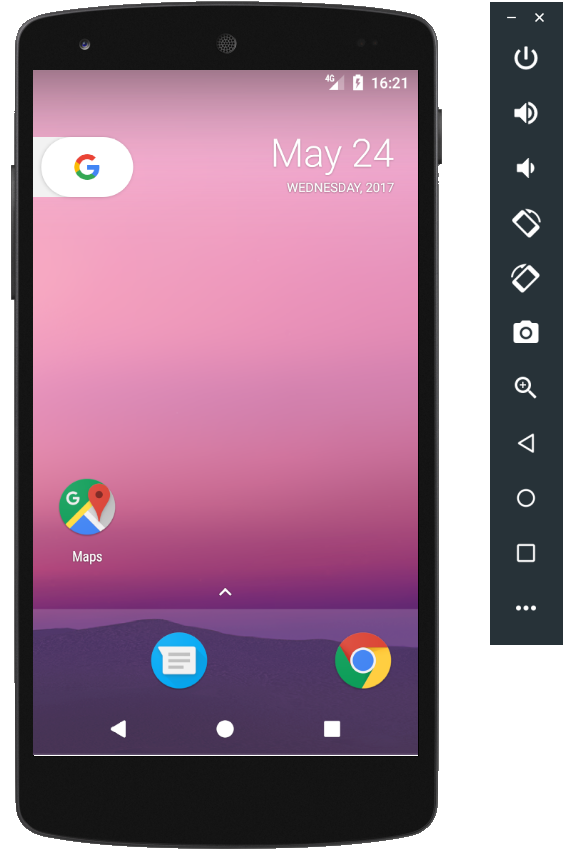
\includegraphics[width=1\textwidth]{figures/emulator}
\caption{Android Emulator.}
\label{fig:androidEmulator}
\end{figure}

\noindent
I emulatorens kontrolpanel findes Extended Controls, som fremgår af \autoref{fig:emulatorExtend}. Hertil er det muligt at simulere en smartphones egenskaber, såsom lokalisation.

\begin{figure} [H]
\centering
\includegraphics[width=1\textwidth]{figures/imple/emulatorExtend}
\caption{Android Emulator.}
\label{fig:emulatorExtend}
\end{figure}

\noindent
Strukturen i Android Studio opdeles i \textit{manifests}, \textit{res} samt \textit{java} mapper. \textit{Manifests} mappen indeholder en \textit{AndroidManifest.xml} fil, der er essentiel for, at app'en kan køre og indeholder de aktiviter, der implementeres. Derudover er der i denne fil defineret tilladelser for den givne app. For udvikling af app'en har det været nødvendigt at tillade brug af internet samt GPS-lokation, for således at kunne tilgå databasen og beregne afstand i relation til konditionstræningen. 
\textit{Res} mappen indeholder ikke-kode ressourcer, der eksempelvis er de forskellige layouts, som udgør grænsefladerne.
Javaklasserne, der er oprettet i forbindelse med udviklingen af app'en er placeret i \textit{java} mappen.\cite{android2017}
 
\section{Database}
Til implementering af databasen samt kommunikation med denne benyttes programmet XAMPP. Programmet opretter en lokal apache webserver samt database på en given computer, der fungerer som et Localhost miljø. Den lokale webserver simulerer en ekstern webserver, hvilket giver et passende miljø til at teste og udvikle prototypen. Dertil anses dette ikke som værende fjernt fra et virkelighedsnært scenarie, hvor systemet benyttes med ekstern server og database.
Ved direkte håndtering af databasen benyttes phpMyAdmin, der er et online databaseadministrationssystem, som understøtter Structured Query Language (SQL) \cite{silbershatz2011}. 
Databasen er implementeret under navnet \textit{db\_KOL}, hvori tabeller oprettes på baggrund af design jf. \autoref{sec:ER} i relation til attributter og datatyper.

\subsection{Kommunikation med databasen}
Kommunikation mellem Android Studio og databasen kan ikke forekomme direkte, hvorfor php: Hypertext preprocessor scripts benyttes. Php er et Server-Side Scripting Language, hvilket køres på serveren og muliggør, at systemet kan tilgå databasen \cite{silbershatz2011}. Dertil kan de oprettede php-scripts betragtes som databasecontrolleren designet i \autoref{sec:databaseDesign}.
Der er oprettet et php-script, \textit{config.php}, der indeholder informationerne host, bruger, adgangskode samt navn på den oprettede database. Dette script inkluderes i et seperat script, \textit{DB\_connect.php}, til at etablere forbindelsen til databasen. Der er opstillet forskellige php-scripts, som javakoden refererer til via URL links. Af disse links fremgår ip-adressen for serveren samt filplaceringen af det givne script. 

De forskellige scripts får information fra app'en for således at kunne udføre SQL-kommandoer. Informationen sendes fra app'en som en JavaScript Object Notation (JSON) repræsentation. JSON benyttes ved dataoverførsel, det er hertil muligt at pakke data som et objekt eller array.\cite{silbershatz2011} Php-scripts brugt i dette projekt er sat op til at tjekke, hvorvidt der bliver sendt en værdi i det respektive navn. Er værdierne sat og ikke NULL, ligges værdierne i en ny variabel. Et eksempel af dette ses af \autoref{fig:phplogind}, hvor et udklip af php-scriptet for log ind er visualiseret. 

\begin{figure} [H]
\centering
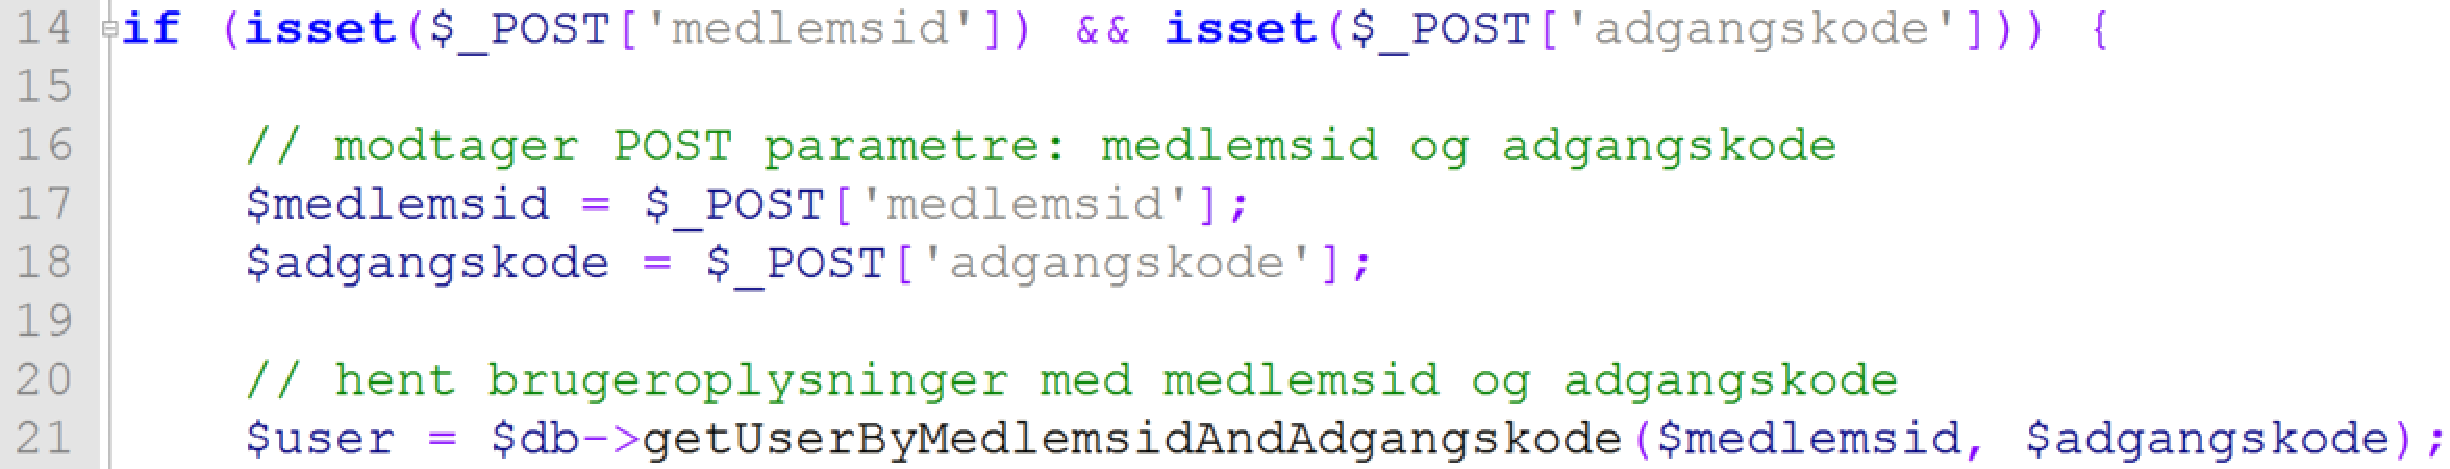
\includegraphics[width=1\textwidth]{figures/imple/phplogind}
\caption{Udklip af log ind php-script, hvor medlemsid samt adgangskode modtages og indsættes i tilhørende variabler, der benyttes i et funktionskald.}
\label{fig:phplogind}
\end{figure}

\noindent
Dette udklip viser, hvordan koden modtages og gemmes i nye variabler. Værdierne gemmes i et associativt array, der ved hjælp af en POST-metode gør det muligt at overføre data til et andet script, \textit{db\_functions.php}, hvori SQL-kommandoer udføres \cite{w3schools2017}. Linje 21 viser, hvordan variablerne benyttes i et funktionskald, der eksekveres i \textit{db\_functitons.php}. Af \autoref{fig:phplogindsql} ses et udklip af denne funktion.

\begin{figure} [H]
\centering
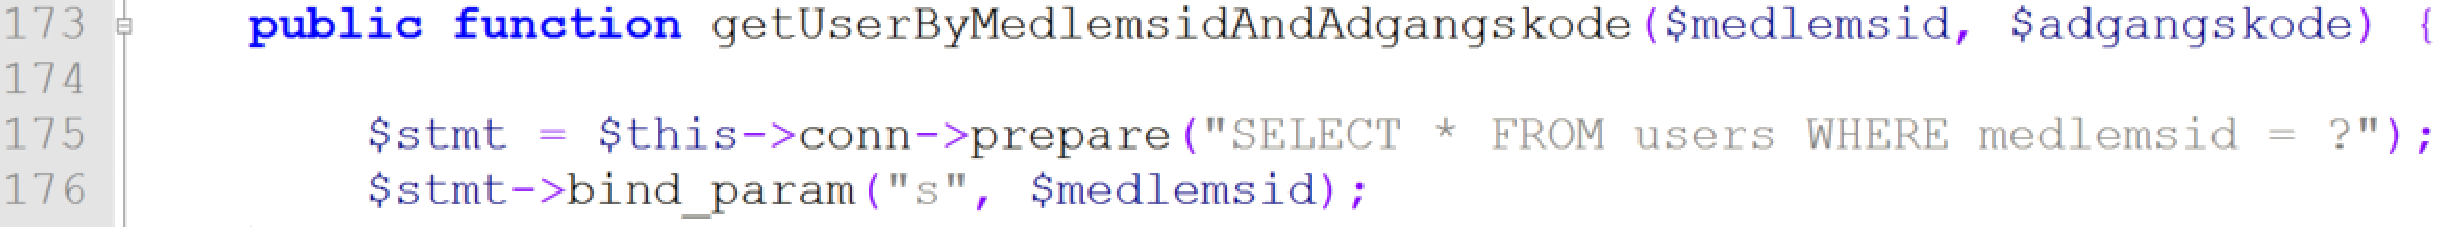
\includegraphics[width=1\textwidth]{figures/imple/phplogindsql}
\caption{Udklip af php-scripts for funktionen log ind. Herunder ses SQL-kommandoen for denne funktion.}
\label{fig:phplogindsql}
\end{figure}

\noindent
Det ses af \autoref{fig:phplogindsql}, hvordan en SQL-kommando udføres. Den viste SQL-kommando henter alt fra tabellen \textit{users} tilhørende medlemsid'et i databasen, der er lig spørgsmåltegn. Spørgsmåltegnet markerer et bindingspunkt, hvorpå en parametre kan tilknyttes. Parameteren, der bindes på ved brug af \textit{bind\_param}, fremgår af linje 176, hvoraf \textit{"s"} indikerer, at medlemsid'et er af typen string. I dette tilfælde valideres log ind-informationerne førend user returneres til log ind php-scriptet, der håndterer user, hvilket fremgår af \autoref{fig:phplogindresp}.


\begin{figure} [H]
\centering
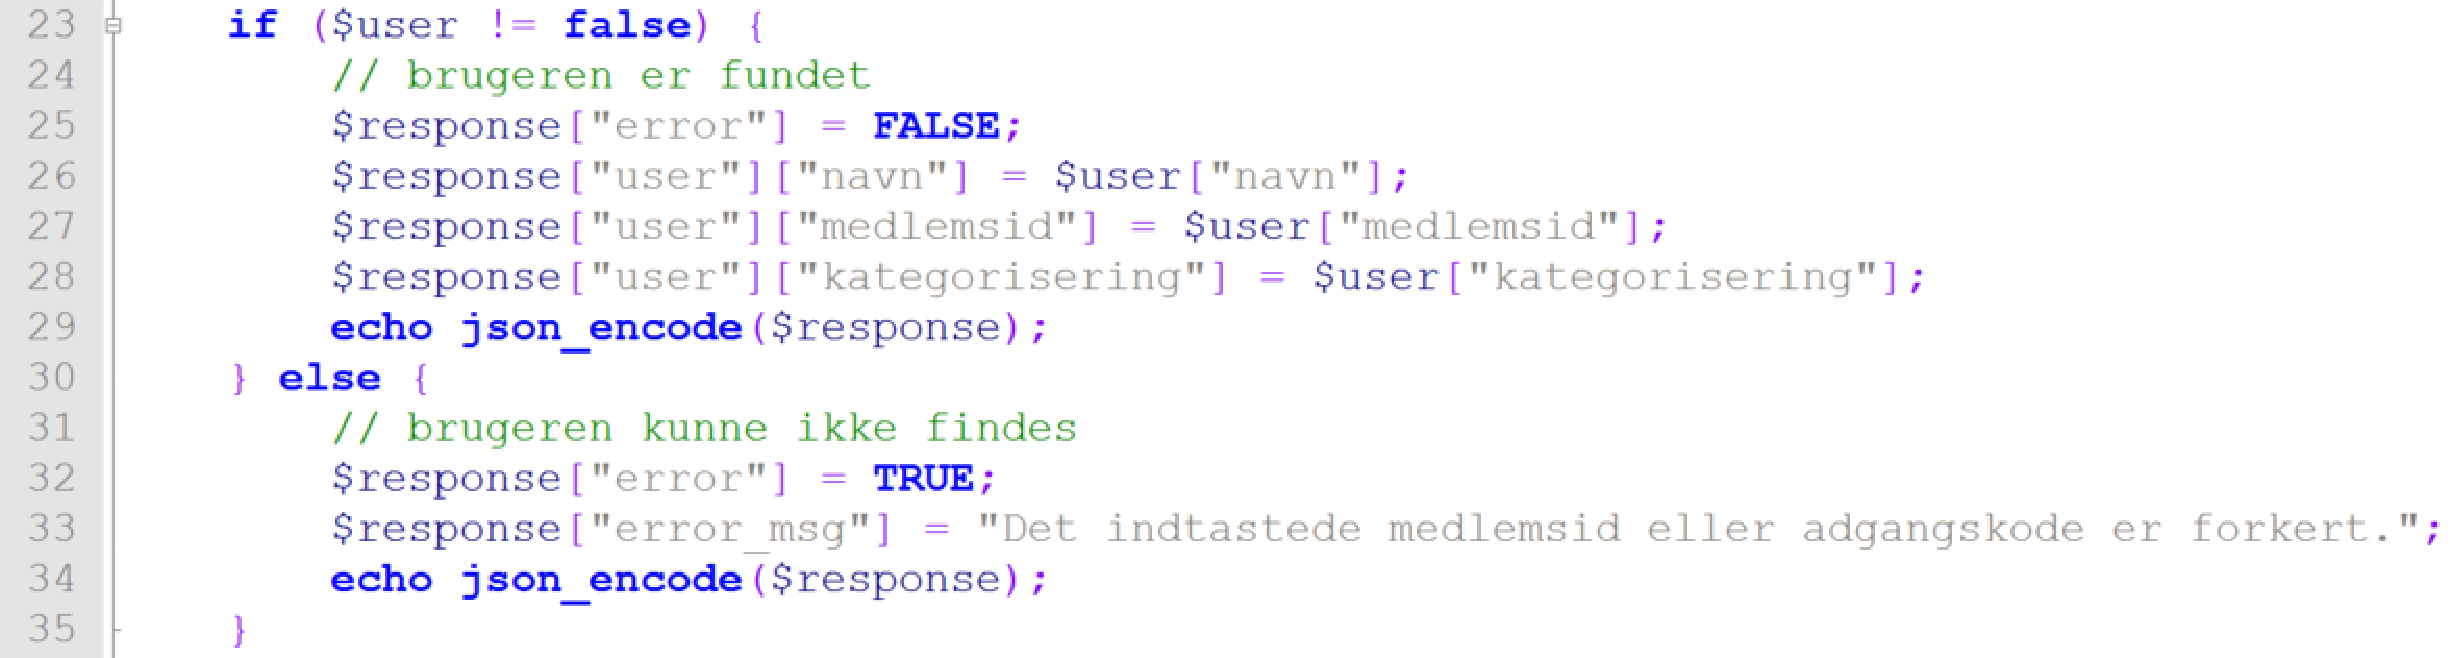
\includegraphics[width=1\textwidth]{figures/imple/phplogindresp}
\caption{Udklip af php-scripts, hvori user håndteres og sendes til app'en.}
\label{fig:phplogindresp}
\end{figure}

\noindent
Som det ses af \autoref{fig:phplogindresp} opstilles if/else statement, der håndterer, hvorvidt \textit{user} returneres. Hvis \textit{user} returneres bliver brugerdata gemt i \textit{response}, der sendes tilbage til app'en som en JSON repræsentation. Returneres \textit{user} ikke, gemmes en fejlmeddelelse i \textit{response}, der ligeledes sendes til app'en som en JSON repræsentation. 

Der er i javakoden opsat en \textit{Response.listener}, der lytter efter respons. Ved respons oprettes et nyt JSON objekt, hvori responset lagres, således dette kan benyttes i app'en. 


\section{Grænseflader}
Til at implemtere grænseflader i systemet benyttes XML-filer, der håndteres i deres respektive controllere. I disse filer er det muligt at definere, hvilken type elementer, der skal indgå i layoutet. Dertil kan typen af layout defineres alt efter, hvordan layoutet skal opstilles. Layouts brugt i dette system er af type linear og relative.  

Elementer, såsom TextView og Button, opstilles i layouts med type, størrelse samt orientering. Forekommer det, at elementerne skal benyttes i javakoden, defineres disse ligeledes med et id. Et eksempel af layoutkode fra log ind ses af \autoref{fig:logindlay}.

\begin{figure} [H]
\centering
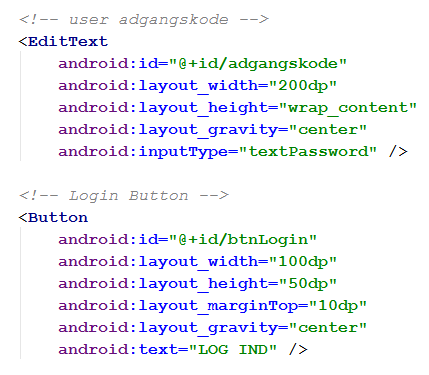
\includegraphics[width=0.6\textwidth]{figures/imple/logindlay}
\caption{Udklip af kode fra log ind-layout. Udklippet viser et \textit{EditText}, hvori brugeren angiver adgangskode samt en Button for log ind.}
\label{fig:logindlay}
\end{figure}

\noindent
Af dette udklip ses koden for tekstfeltet, hvori brugeren angiver adgangskode samt koden for layoutet af log ind-knappen. Feltet for adgangskoden er her af typen \textit{EditText}, der tillader, at brugeren kan angive tekst. Dette felt har ligeledes et id, der muliggøre at referere til feltet og hente den angivne adgangskode til validering af log ind. Knappen er opstillet af typen Button og har ligeledes et id, hvortil en listener er opstillet i javakoden. Dette ses yderligere af \autoref{fig:list}.

\section{Model- og controllerklasser} \label{sec:impmodelcon}
Model- og controllerklasser er implementeret i \textit{Java Class} filer. Heri er klasser defineret med navn samt tilhørende attributter og metoder. Af \autoref{fig:javaclass} ses et eksempel på, hvordan en controller er implementeret. 

\begin{figure} [H]
\centering
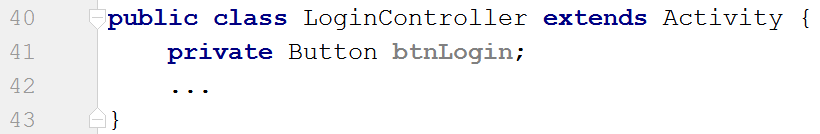
\includegraphics[width=0.6\textwidth]{figures/imple/javaclass}
\caption{Udpluk af javaklassen for LoginController. Punktummerne symboliserer den resterende kode, der ikke anses nødvendig for forklaring af opsætning af javaklasser.}
\label{fig:javaclass}
\end{figure}

\noindent
Det fremgår af dette udklip, at klassen, \textit{LoginController}, er af typen public og nedarver \textit{activity}. Dette gør sig gældende for samtlige klasser implementeret. Denne klasse for \textit{LoginController} har attributten \textit{btnLogin}, der referer til log ind knappen på grænsefladen. Idet app'en skal reagere, når brugeren trykker på btnLogin, opsættes en listener på knappen, hvilket ses af \autoref{fig:list}.


\begin{figure} [H]
\centering
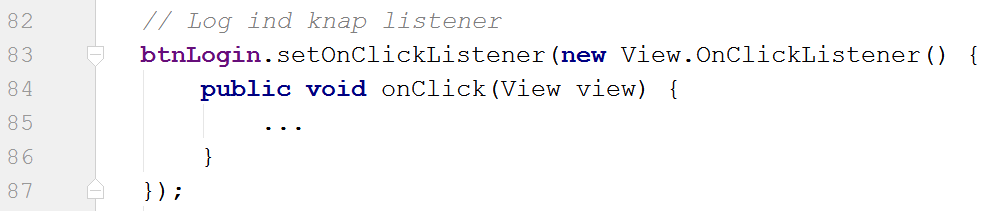
\includegraphics[width=0.6\textwidth]{figures/imple/list}
\caption{Udpluk af koden for listeneren opsat for log ind knappen. Punktummerne symboliserer den resterende kode, der ikke anses nødvendig for forklaring af opsætning af listener.}
\label{fig:list}
\end{figure}


\noindent
Af dette udklip ses den opsatte listener, der har til formål at lytte på knappen. Indenfor listeneren er der opstillet kode, hvilket symboliseres ved punktummer, der køres idet der trykkes på knappen. Denne listener er ligeledes implementeret for samtlige knapper i controllerklasserne. Listeneren er implementeret i controllerklasserne, da det er disse filer, som håndterer input for de tilhørende layouts.

Modelklasserne er implementeret på samme vis som controllerklasserne, de har dog til formål at lagre data forinden det sendes til databasen. I disse klasser er der ligeledes opstillet attributter med tilhørende get- og set-metoder. 

